\chapter{Theoretischer Hintergrund}
\label{chap:theoretischer-hintergrund}
Zum Architekturprinzip der Microservices gibt es bereits eine Vielzahl akademischer Publikationen.
In diesem Kapitel wird in den theoretischen Hintergrund der für diese Thesis relevanten Literatur eingeführt.
Zunächst wird ein kurzer Vergleich zwischen dem häufig verwendeten Legacy-Architekturprinzip \emph{Monolith} und dem behandelten neuen Architekturprinzip \emph{Microservices} gezogen.
Anschließend werden aktuelle Arbeiten zur Migration zu Microservices-Architekturen beschrieben.
Des Weiteren wird das Werkzeug \gls{arh} vorgestellt, das ein wesentlicher Bestandteil und Untersuchungsobjekt dieser Arbeit ist.
Abschließend wird ein Überblick über das Produkt gegeben, das mithilfe des \gls{arh} überarbeitet werden soll.

\section{Vergleich von monolithischen und Microservices-Systemen}

Die monolithische Systemarchitektur hat lange Zeit einen Großteil der Softwareprodukte ausgemacht und ist die simpelste Art, Software zu entwickeln.
Die gesamte Funktionalität eines Monolithen befindet sich in einer Applikation, die in sich selbst geschlossen ist.
Auch wenn in dieser Arbeit die Migration weg von dieser Architektur thematisiert wird, hat sie ihre Stärken.
Da es sich um eine sehr einfache Architektur handelt, können kleine Anwendungen sehr schnell erstellt, getestet und zum Laufen gebracht werden.
Es wird kein kompliziertes Kommunikationsmodell benötigt, da Monolithen oft in einer Programmiersprache und sogar mit nur einem Framework geschrieben werden.

Je größer Monolithen jedoch werden, desto stärker zeigen sich die Schwächen dieser Architektur.
Es entstehen riesige Codebasen und kleine Änderungen erzwingen erneutes Bauen und Testen der gesamten Applikation.
Das steht auch dem modernen agilen Arbeitsprinzip im Weg.
Wenn nur einzelne Komponenten eines Monolithen eine hohe Last erfahren, muss trotzdem das gesamte System skaliert werden, was zu einer Verschwendung von Rechenleistung führen kann und die Anwendung ineffizient macht.

Die meisten dieser Probleme werden durch die Microservices-Architektur gelöst.
Dabei besteht ein System aus vielen kleinen (Micro-) Services.
Diese zeichnen sich dadurch aus, dass sie möglichst klein gehalten werden, genau eine Aufgabe haben und unabhängig ausgeführt werden können \cite{10220070}.
Durch die Entkopplung der Services wird im Gegensatz zu Monolithen ein Kommunikationsmodell zwischen den Services nötig.
Dafür existieren verschiedene Lösungen, die im Rahmen dieser Arbeit näher betrachtet werden.
Ein sehr häufig benutztes ist beispielsweise \gls{rest}.

Die Vorteile dieser Architektur gegenüber Monolithen sind vielseitig.
Da die Services unabhängig voneinander entworfen sind, können sie einzeln implementiert, getestet und gebaut werden.
Dies erleichtert die Automatisierung des Bauens und Testens durch \gls{ci} / \gls{cd}.
Außerdem können Services abhängig von der Last einzeln skaliert werden, was die Effizienz in bestimmten Szenarien deutlich erhöht.
Darüber hinaus sind Entwickler flexibel in der Wahl der Programmiersprache und des Frameworks für einzelne Services, da die einzige Anforderung die Berücksichtigung des gewählten Kommunikationsmodells ist.

Wie bereits erwähnt, gibt es allerdings auch Punkte, in denen Monolithen vorteilhafter sind, sodass eine Microservices-Architektur nicht universell den Monolithen vorzuziehen ist.
Dazu gehört vor allem die Komplexität des Systems, die bei einer Microservices-Architektur deutlich höher ist.
Dies liegt an der Aufteilung in einzelne Services, die ein ausgefeiltes Kommunikationsmodell erfordern.
Die Kommunikation zwischen den Komponenten ist in jedem Fall langsamer und ineffizienter als bei Monolithen, bei denen lediglich Funktionen im selben ausgeführten Programm aufgerufen werden.

\section{Migration zu Microservices}

Aufgrund der genannte Vorteile der Microservices-Architektur gegenüber Monolithen, besteht großes Interesse daran, Monolithen zu Microservices zu migrieren.
Der Eingriff in tiefe Architekturprinzipien eines Systems ist natürlich keine einfache Operation.
Deswegen ist die Migration zu Microservices seit einiger Zeit ein stark untersuchtes Thema.

Anwendungen können eine unterschiedliche Ausgangsarchitekturen haben.
Es gibt viele verschiedene Migrationsmethoden, die wissenschaftlich untersucht wurden, sodass es für jedes System eine passende gibt.

Für den gesamten Prozess der Migration zu Microservices gibt es im Wesentlichen drei verschiedene Methoden \cite{master-daniel-koch}:
\begin{enumerate}
	\item \textbf{Re-Factor:} Der existierende Code wird kontinuierlich verändert, ohne die Funktionalität der Anwendung zu verändern.
	\item \textbf{Re-Build:} Die gesamte Anwendung wird im Rahmen der Architekturveränderung verändert. Dabei werden passend zu den Anforderungen neue Technologien verwendet.
	\item \textbf{Neue Anwendung:} Eine völlig neue Anwendung wird von Grund auf entwickelt.
\end{enumerate}

Doch keine davon bietet genug Flexibilität, um alle Anwendungsfälle abdecken zu können.

\section{\acrfull{mmf}}
\label{sec:mmf}

Aufgrund der beschriebenen Vorteile von Microservices Architekturen ist es im Interesse vieler Unternehmen und Entwickler, existierende Applikationen und Systeme mit monolithischer Architektur zu Microservices-basierten Systemen zu migrieren.
Der Planungsprozess dieser Migration ist allerdings sehr zeit- und kostenintensiv und durch große Risiken geprägt, da dabei Systeme sehr tiefliegend verändert werden.
Erschwert wird er durch das Fehlen klarer und strukturierter Anleitungen.
Es wurde bereits durch mehrere Metastudien versucht, eine Übersicht über verschiedene Refactoring- und Migrationsverfahren zu geben, die für Entwickler hilfreich sein kann.
Jedoch bleibt dabei das Problem bestehen, dass sich der aktuelle Stand der Literatur schnell ändert und Metastudien dadurch teilweise obsolet werden.
Dieses Problem könnte durch die Umsetzung der Anleitung in Form eines Werkzeugs, das Entwickler bei der Migration unterstützt, gelöst werden.
Im Gegensatz zu Metastudien könnte dieses Werkzeug dynamisch an den neuesten Forschungsstand angepasst werden.

Aus diesem Grund hat das \gls{ese} das Werkzeug \gls{arh} \cite{arh-github} entwickelt, das in diesem Kapitel vorgestellt wird.
Während \Citet{fritzsch2022architecturecentric} den Entwurf des Frameworks für das Werkzeug beschreiben, wurde das Werkzeug im Rahmen von zwei Masterarbeiten entwickelt \cite{master-daniel-koch}\cite{master-tobias-haller}.
Der \gls{arh} ist eine web-basierte Anleitung, die Entwickler durch drei Phasen der Migrationsplanung führt.
Eine Übersicht über diese Phasen und die Funktionsweise des Werkzeugs ist in \cref{fig:arh-overview} zu sehen.
Im Folgenden werden diese drei Phasen genauer beschrieben:

\begin{itemize}
	\item \textbf{Phase 1: System Comprehension:}
	In Phase 1 wird das Verständnis des Systems, das migriert werden soll, angestrebt.
	Mit den Stakeholdern sollen dabei strategische Ziele für Produkt und Unternehmen definiert, sowie Qualitätsmerkmale und gewünschte Szenarien identifiziert werden.
	Es sollen sich dadurch mögliche Treiber für die neue Microservices-Architektur herauskristallisieren.
	Durch das resultierende Verständnis des Systems wird ein Vergleich der alten monolithischen Architektur und einer potentiellen neuen Microservices-Architektur möglich.
	Architekten sollen dann mithilfe dieser Informationen eine Entscheidung für oder gegen die Migration zu Microservices fällen.
	\item \textbf{Phase 2: Strategy Definition:}
	Falls sich in Phase 1 für die Migration zu Microservices entschieden wurde, wird in Phase 2 die Planung der Migration begonnen.
	Eine der zwei hauptsächlichen Aufgaben in dieser Phase ist die konkrete Definition, welche Migrationsstrategie benutzt werden soll, um das System zu modernisieren.
	Dafür kann zwischen (momentan) 22 verschiedenen Methoden gewählt werden, die aus akademischen Publikationen stammen.
	Das Werkzeug kann Entwickler dabei unterstützen, indem es aufgrund der Eingaben aus Phase 1 empfohlene Methoden vorschlägt.
	Der zweite Teil dieser Phase besteht darin, einen Service-Identifikationsansatz zu wählen.
	Durch diesen kann in der nächsten Phase eine sinnvolle Aufteilung in einzelne Services bestimmt werden.
	\item \textbf{Phase 3a: Architecture Definition:}
	Phase 3 ist in zwei Teile aufgeteilt.
	Im ersten Abschnitt wird die neue Architektur definiert.
	Hier wird, basierend auf der Methode zur Migration, die in der Planungsphase gewählt wurde, die Identifikation von Microservice-Kandidaten realisiert.
	Außerdem wird allgemeiner die Architektur des gesamten Systems geplant, wobei das Werkzeug Entwickler durch eine Liste von vorgeschlagenen Patterns und Best Practices unterstützen kann.
	 Phase 3a und 3b sind eng verbunden, denn durch Erkenntnisse in der Implementierung kann die Planung häufig noch mehrmals überarbeitet werden und dadurch eine neue Implementierung begonnen werden.
	\item \textbf{Phase 3b: Service Implementation:} In Phase 3b startet dann ein Zyklus von Implementierungen der in Phase 3a definierten Services.
	Bei Implementierung selbst kann das Werkzeug Entwickler nicht unterstützen.
	Doch Bestandteil der Entwicklungszyklen ist auch, dass das entstehende System anhand der Qualitätsmerkmale zu bewerten.
	Dadurch kann eine unpassende Architekturdefinition oder auch eine unpassende Aufteilung in Services frühzeitig erkannt und korrigiert werden.
	Ist diese Phase abgeschlossen, ist eine erste Version des migrierten Systems fertig.
\end{itemize}

\begin{figure}
	\centering
	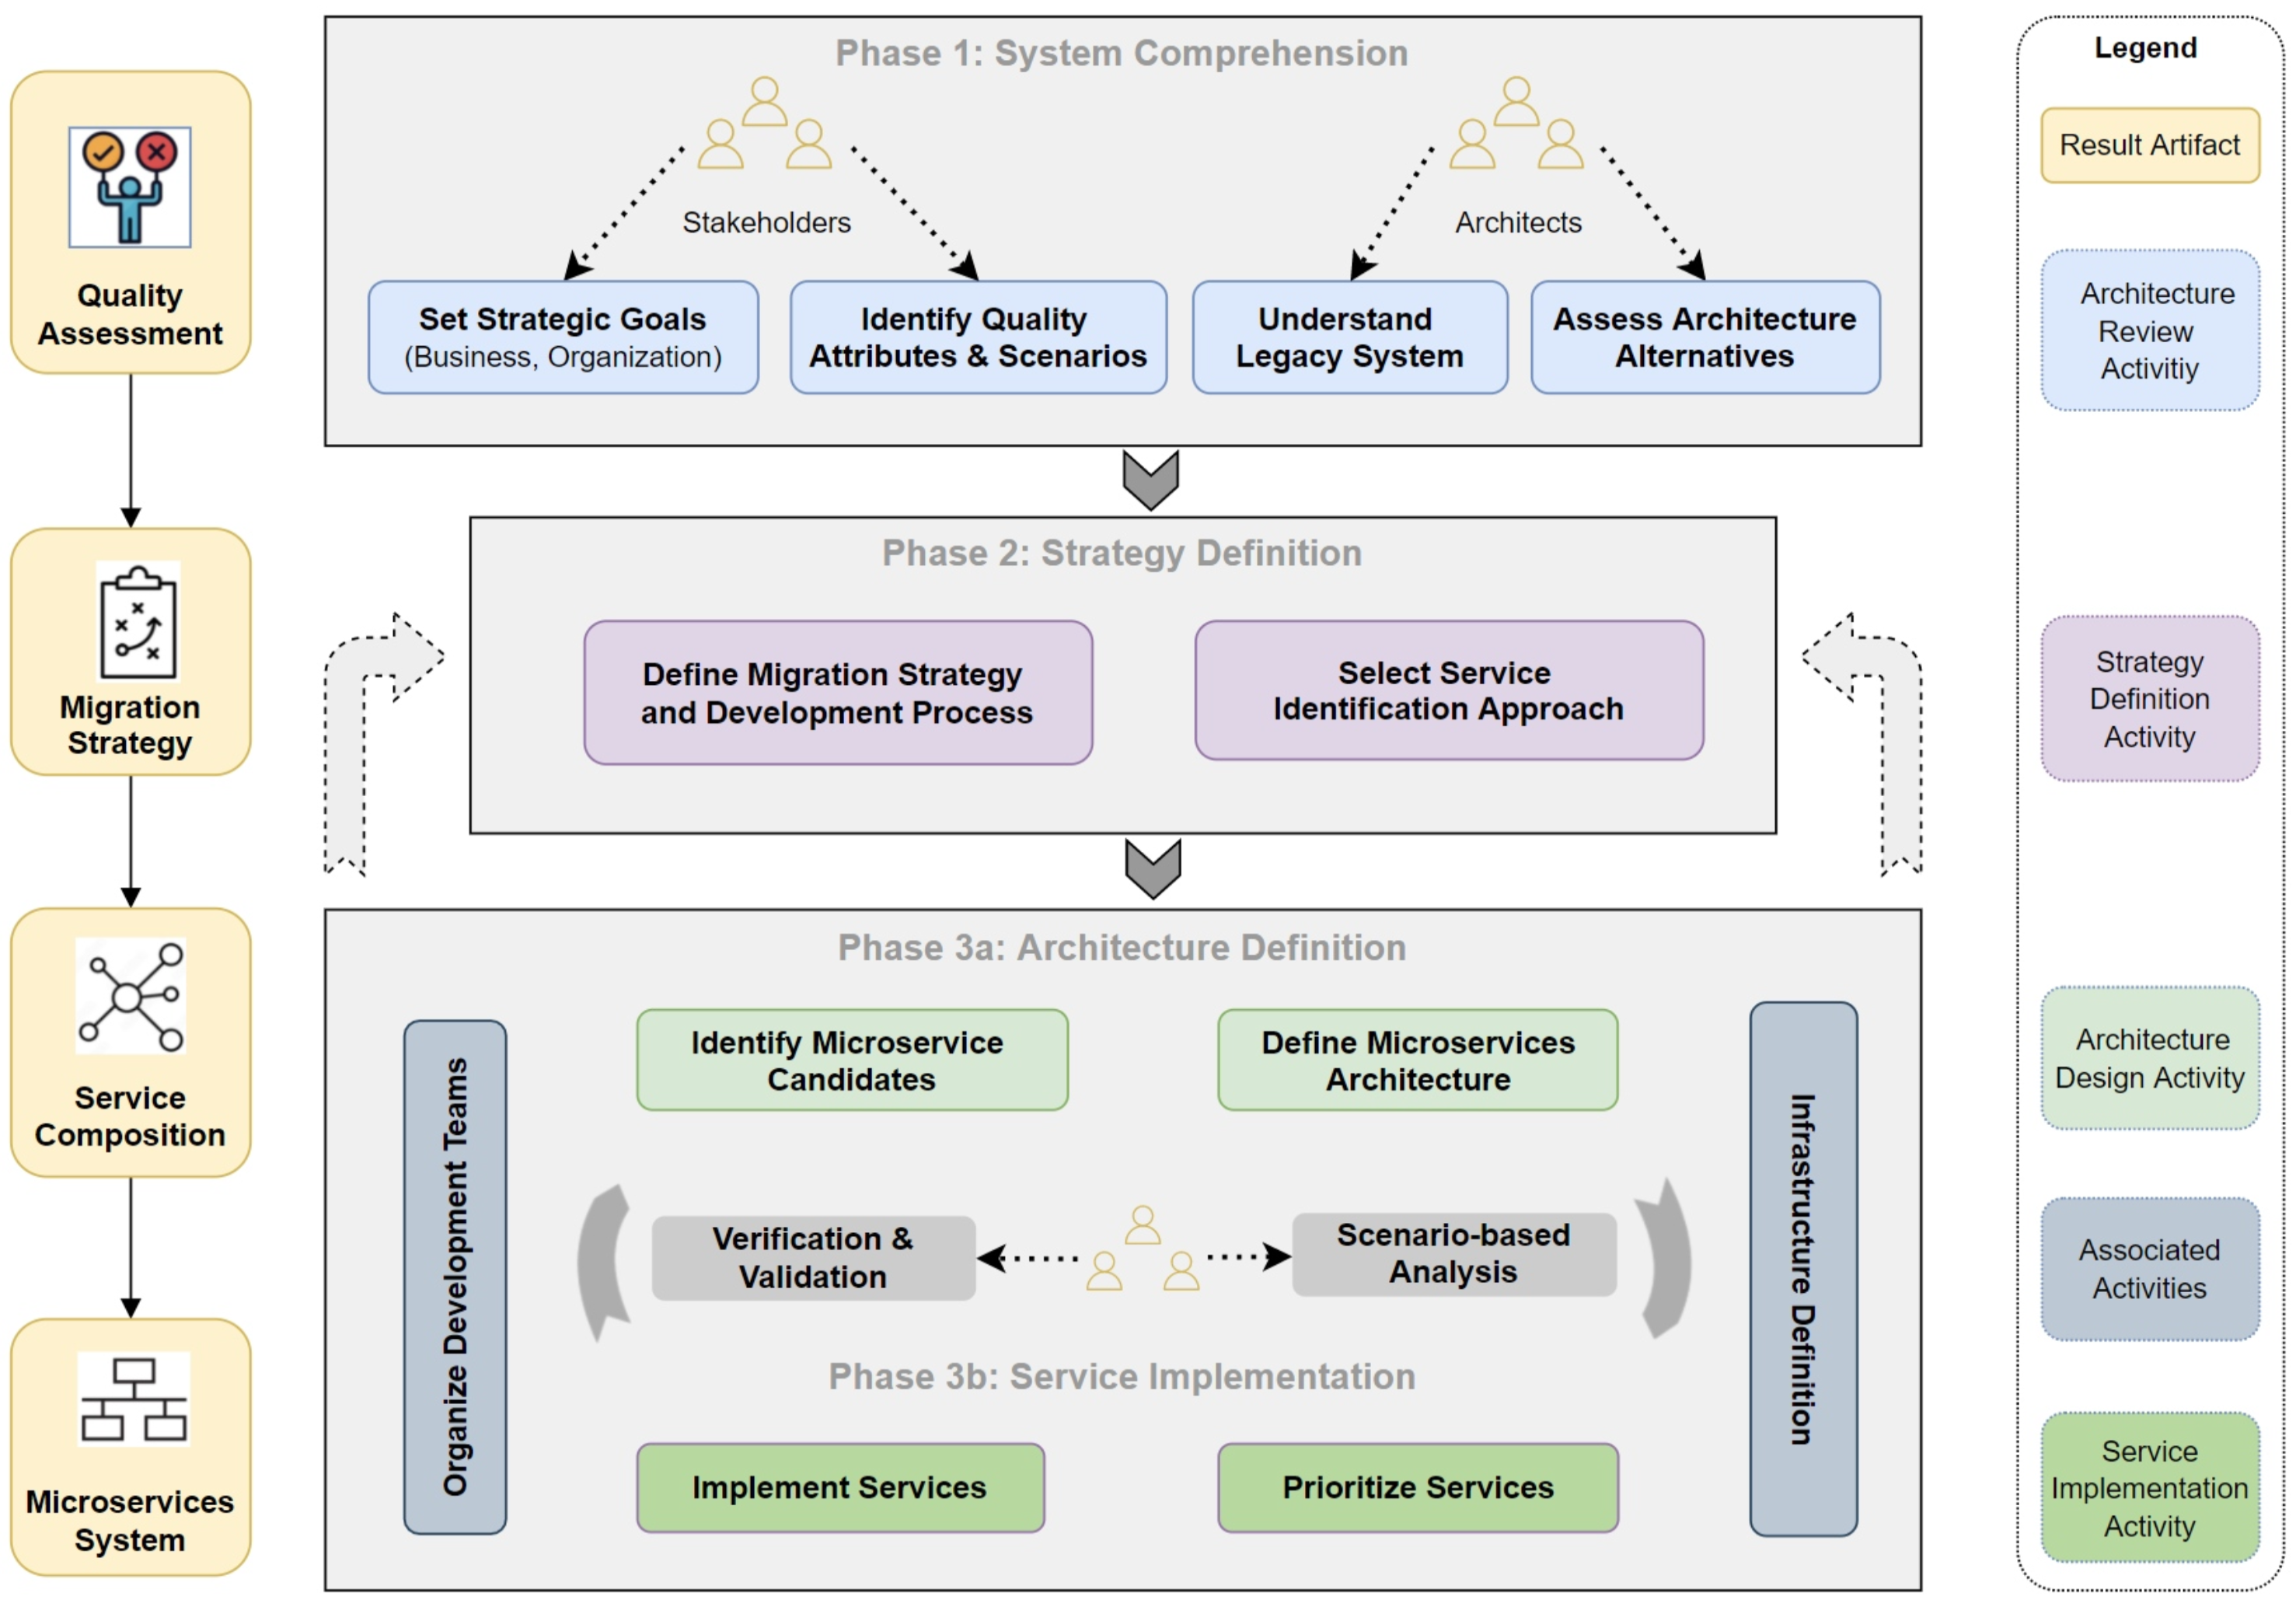
\includegraphics[width=\textwidth]{figures/mmf-overview}
	\caption[Architecture Refactoring Helper Übersicht]{
		Übersicht über den \acrlong{arh} des \gls{ese} \cite{fritzsch2022architecturecentric}. Es sind die drei Phasen des Prozesses zu erkennen, sowie einige Schritte der einzelnen Phasen.
	}
	\label{fig:arh-overview}
\end{figure}

\section{jadice flow}

Das vorgestellte Werkzeug soll in dieser Thesis nun erstmals in der Industrie benutzt werden.
Deswegen wird in diesem Abschnitt näher auf das Produkt \emph{jadice flow} eingegangen, das damit überarbeitet werden soll.

\emph{jadice flow} ist ein Produkt der Firma \emph{levigo solutions}\footnote{\url{https://solutions.levigo.de/}}.
\emph{levigo solutions} beschäftigt über 30 Mitarbeiter, von denen ungefähr sechs seit vier Jahren an \emph{jadice flow} arbeiten.
\emph{jadice flow} basiert bereits auf einer Microservices-Architektur, ist jedoch erst die erste Generation nach der Überführung des vorherigen Monoliths \emph{jadice server}\footnote{\url{https://jadice.com/produkte/server/}}.
Beide Produkte bieten Workflow-basierte Dokumentenverarbeitung an, bei der mit komplexen Datenströmen umgegangen werden kann.
Durch den Umstieg auf eine Microservices-Architektur können in der neuen Generation einzelne Verarbeitungsschritte skaliert werden.
Der Großteil der Services ist in Java geschrieben, doch durch den Betrieb in Containern ist jadice flow prinzipiell unabhängig von der Programmiersprache.

Einen beispielhaften Workflow stellt der \emph{E-Mail converter} dar.
Dabei werden E-Mails in Einzelteile aufgeteilt (Körper, Anhänge) und diese dann einzeln in das Zielformat konvertiert.
Die einzelnen Arbeitsschritte dabei können parallelisiert werden und separat skaliert werden.
Am Ende werden die Ergebnisse kombiniert.
Im Gegensatz zu einfacher PDF-Darstellung von E-Mails in geläufigen Programmen bietet \emph{jadice flow} zusätzliche Features, wie die tiefe Analyse und Darstellung von Archiven in Anhängen.

Da \emph{jadice flow} die erste Generation in Microservices-Architektur ist, wird noch einiges Verbesserungspotential vermutet.
Durch die Analyse von \emph{jadice flow 1.0} mithilfe des Werkzeugs und weiterer Forschung im Rahmen dieser Bachelorarbeit soll ein Refactoring-Prozess für \emph{jadice flow 2.0} angestoßen werden.

Da das Framework für die Anwendung auf Monolithen gedacht ist, soll in dieser Arbeit die Anwendung des Frameworks auf ein bereits migriertes System angewendet werden, um dessen Eigenschaften weiter zu verbessern.
Dadurch wird erforscht, inwiefern sich Framework und Werkzeug auf eine bereits existierende Microservice-Architektur anwenden lassen.
Falls es deshalb für diesen Anwendungsfall zielführend ist, wird zusätzlich die ursprüngliche monolithische Anwendung von \emph{jadice flow} (\emph{jadice server}) hinzugezogen.
Die Ergebnisse dessen könnten dann mit \emph{jadice flow} verglichen werden.

\section{Ähnliche Forschung}

In dieser Thesis wird sehr vordergründig das Microservices Migration Framework des ESE  untersucht.
Dieses ist aufgrund vorheriger Arbeiten wie \Citet{10.1007/978-3-030-06019-0_10} entstanden.

In 2019 kategorisieren \Citet{10.1007/978-3-030-06019-0_10} zehn verschiedene Migrations-Methoden.
Dabei wird ein Mängel an praktisch anwendbaren Methoden hervorgehoben, die gute Werkzeugunterstützung und Metriken zur Verifikation der Ergebnisse bieten.

Als Folge darauf stellen \Citet{fritzsch2022architecturecentric} 2022 dann die Planung ein solchen Frameworks vor. Der Migrationsprozess mit Framework und dessen Arbeitsweise in drei Phasen wird bereits beschrieben. Auch wird die Entwicklung eines Web-basierten Werkzeugs erwähnt, das das Framework benutzt und Entwickler bei der Migration unterstützt.

\Citet{10.1145/3242163.3242164} beschreiben geläufige Gefahren bei der Migration zu Microservices-Architekturen.
Dabei  werden fünf architektonische Fehlermuster und vier Fehlermuster bei der Migration aufgeführt.
Außerdem werden Lösungsmöglichkeiten für jedes Muster beschrieben.

%\section{Refactoring}
%
%Obwohl in dieser Thesis ein Framework zur Migration zu Microservices im Mittelpunkt steht, sieht man schnell, dass die Migration eng verwandt mit dem Refactoring ist.
%Deswegen werden folgend ein paar Quellen vorgestellt, die das Refactoring von Microservices-Architekturen behandeln.
%
%\Citet{https://doi.org/10.1002/spe.2974} beschreiben in einem Artikel zur $\mu$TOSCA toolchain, wie sie mit dem  $\mu$TOSCA Modell Architekturen von Microservices-basierten Systemen mit dem OASIS Standard TOSCA darstellen können.
%Außerdem beschreiben sie die Möglichkeit, das $\mu$TOSCA Modell eines Systems durch das zugehörige Kubernetes Deployment automatisch zu ermitteln.
%Das $\mu$TOSCA Modell einer Applikation soll dann dazu genutzt werden, potentielle architektonische Probleme zu finden.
%Für das Ermitteln des $\mu$TOSCA Modells und das Identifizieren von Architektur Smells stellen sie zwei Werkzeug Prototypen ($\mu$Miner und $\mu$Freshener) vor.

